\chapter{Lesson 1}
\section{Introduction}
The web has a vast number of resources available for learning how to play
guitar. You can learn how to play songs, how to repair your broken instrument,
how to play fancy scales, and much more. The trouble is, there just aren't many
GOOD guitar lessons available to someone looking to start playing guitar. These
guitar lessons are designed for people who own (or have borrowed) a guitar, but
don't yet know the first thing about playing it.

\subsection{What you'll need for these Guitar Lessons}
%
\begin{itemize}
\item A guitar with six strings. Any type of guitar will work fine.
\item A guitar pick. Medium gauged picks are recommended to start with, but any
      will work okay in a pinch.
\item A chair without arms.
\item A reasonable amount of patience.
\end{itemize}
%
\subsection{Guitar Lesson Overview: What you'll learn}
By the end of this guitar lesson, you will have learned: the names of many
parts of the guitar, the names of the open strings, the process of tuning the
guitar, how to hold and use a pick, how to play a chromatic scale, and how to
play a simple song using Gmajor, Cmajor, and Dmajor chords. 

\section{Parts of a Guitar}
\begin{wrapfigure}{l}{80mm}
% add the image describing the parts of a guitar
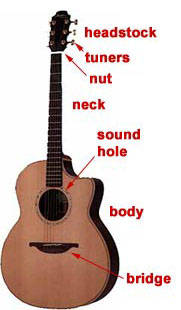
\includegraphics{partone/partsofaguitar.jpg}
\end{wrapfigure}

Although there are many different types of guitars (acoustic, electric,
classical, electric-acoustic, etc.), they all have many things in common. The
diagram to the left illustrates the various parts of a guitar.

At the top of the guitar in the illustration is the \term{headstock}, a general term
which describes the part of the guitar attached to the slimmer neck of the
instrument. On the headstock are \term{tuners}, which you will use to adjust the
pitch of each of the strings on the guitar.

At the point in which the headstock meets the neck of the guitar, you'll find
the \term{nut}. A nut is simply a small piece of material (plastic, bone, etc.), in
which small grooves are carved out to guide the strings up to the tuners.

The neck of the guitar is the area of the instrument you'll concentrate a great
deal on: you'll put your fingers on various places on the neck, in order to
create different notes.

The neck of the guitar adjoins the \term{body} of the instrument. The body of the
guitar will vary greatly from guitar to guitar. Most acoustic and classical
guitars have a hollowed out body, and a \term{sound hole}, designed to project the
sound of the guitar. Most electric guitars have a solid body, and thus will not
have a sound hole. Electric guitars will instead have \term{pick-ups} where the
soundhole is located. These \term{pick-ups} are essentially small microphones, which
allow the capture the sound of the ringing strings, allowing them to be
amplified.

The strings of the guitar run from the tuning pegs, over the nut, down the
neck, over the body, over the sound hole (or pick-ups), and are anchored at a
piece of hardware attached to the body of the guitar, called a \term{bridge}. 

\section{The neck: A closer look}
\begin{wrapfigure}{l}{50mm}
% insert image of the neck
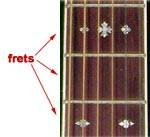
\includegraphics{partone/frets.jpg}
\end{wrapfigure}

Examine the neck of your guitar. You'll notice there are metal strips running
across it's entire surface. These pieces of metal are referred to as \term{frets} on
a guitar. Now, here's what you'll need to keep in mind: the word \term{fret} has two
different meanings when used by guitarists. It can be used to describe:
%
\begin{enumerate}
\item The piece of metal itself
\item The space on the neck between one piece of metal and the next 
\end{enumerate}
%
To further explain, the area of the neck between the nut and the first strip of
metal is referred to as the \term{first fret}. The area on the neck between the
first and second strip of metal is referred to as the \term{second fret}. And so
on\ldots{} 

\section{Holding a Guitar}
Now, that we know about the basic parts of a guitar, it's time to get our hands
dirty, and start learning to play it. Get yourself an armless chair, and take a
seat. You should be sitting comfortably, with your back against the back of the
chair. Slouching significantly is a no-no; you'll not only end up with a sore
back, you'll develop bad habits on the guitar.

Now, pick up your guitar, and hold it so the back of the body of the instrument
comes in contact with your stomach/chest, and the bottom of the neck runs
parallel to the floor. The thickest string on the guitar should be the closest
to your face, while the thinnest should be closest to the floor. If this isn't
the case, turn the guitar the in other direction. Typically, a right-handed
person will hold the guitar so the headstock points to the left, whereas a
left-handed person will hold the guitar so the headstock points to the right.
(NOTE: to play the guitar as a lefty would, you will need a left-handed
guitar.)

When playing the guitar sitting down, the body of the guitar will rest on one
of your legs. In most styles of guitar playing, the guitar will rest on the leg
farthest away from the headstock. This means, a person playing the guitar in a
right-handed fashion will typically rest the guitar on his/her right leg, while
someone playing the guitar in a lefty manner will rest it on their left leg.
(NOTE: proper classical guitarist technique dictates the exact OPPOSITE of the
above, but for this lesson, let's stick to our initial explanation)

Next, concentrate on your \term{fretting hand} (the hand closest to the neck of the
guitar, when sitting in proper position). The thumb of your fretting hand
should rest behind the neck of the guitar, with your fingers in a slightly
curled position, poised above the strings. It is extremely important to keep
these fingers curled at the knuckles, except when specifically instructed not
to do so. 

\section{Holding a Pick}
\begin{wrapfigure}{l}{50mm}
%insert image of the pick
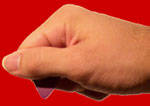
\includegraphics{partone/howtoholdapick.jpg}
\end{wrapfigure}

Hopefully, you've found, bought or borrowed a guitar pick. If not, you'll need
to buy yourself some. Don't be stingy, go and pick up at least 10 of them -
guitar picks are easy to lose (they often don't cost more than 30 or 40 cents
each). You can experiment with different shapes and brands, but I highly
recommend medium gauge picks to start; ones that aren't too flimsy, or too
hard.

The following documentation explains how to hold, and use a pick. When reading,
keep in mind that your \term{picking hand} is the hand which is nearest to the
bridge of the guitar, when sitting in the correct position.

\begin{enumerate}
\item Open your picking hand, and turn the palm to face you.
\item Close your hand to make a very loose fist. Your thumb should remain
      beside your index finger.
\item Rotate your hand until you are looking at it's profile, with your thumb's
      knuckle facing you.
\item With your other hand, slide your guitar pick between your thumb and index
      finger. The pick should be approximately located behind the knuckle of the
      thumb.
\item Be sure the pointed end of the pick is pointing directly away from your
      fist, and is protruding by about a half an inch. Hold the pick firmly.
\item Position your picking hand over the soundhole of your acoustic guitar, or
      over the body of your electric guitar. Your picking hand, with thumb knuckle
      still facing you, should hover over the strings.
\item Do not rest your picking hand on the strings or body of the guitar.
\item Using your wrist for motion (rather than your entire arm), strike the
      sixth (lowest) string of your guitar in a downward motion. If the string
      rattles excessively, try striking the string a bit softer, or with less of the
      pick surface.
\item Now, pick the sixth string in an upwards motion.
\item Repeat the process several times. Try and minimize motion in your picking
      hand: one short picking stroke downwards, then one short picking stroke
      upwards. This process is referred to as \term{alternate picking}
\item Try the same exercise on the fifth, fourth, third, second, and first strings.
\end{enumerate}
%
\subsection{Tips}
\begin{itemize}
\item Holding the pick in this manner will invariably feel awkward at first.
      You will initially have to pay special attention to your picking hand whenever
      you play guitar.
\item Try and create fluidity in your alternate picking. Your downstrokes
      should sound virtually identical to your upstrokes.
\end{itemize}

\section{Tuning}
Unfortunately, before you begin playing, you'll really need to tune your
guitar. The problem is, it is, at first, a relatively difficult task, one that
becomes much easier over time. If you know of anyone who plays guitar, who
could do the job for you, it is advised that you get them to tune your
instrument. Alternately, you could invest in a guitar tuner, a relatively
inexpensive device which listens to the sound of each string, and advises you
(via a few blinking lights) on what you need to do in order to get the note in
tune.

If neither of these options are realistic for you, however, don't fear. You can
learn to tune your instrument, and with some patience and a bit of practice,
you'll become a pro at doing it.
\href{http://guitar.about.com/od/beginners/ss/how_tune_guitar.htm}{Learn to
tune your guitar}.

\section{Playing a Scale}
\begin{wrapfigure}{l}{50mm}
% insert a picture of a hand
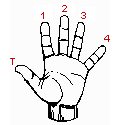
\includegraphics{partone/pickinghand.png}
\end{wrapfigure}

Now we're getting somewhere! In order to become skillful on the guitar, we'll
need to build the muscles in our hands, and learn to stretch our fingers.
Scales are a good, albeit a not very exciting way to do this. Before we start,
look at the diagram above to understand how fingers on the \q{fretting hand} (the
hand that plays notes on the neck) are commonly identified. The thumb is
labelled as \q{T}, the index finger is the \q{first finger}, the middle finger is
the \q{second finger}, and so on. 

\subsection{The Chromatic Scale}
%insert picture of the scale
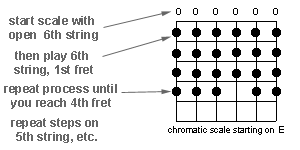
\includegraphics{partone/chromaticscale.png}

The above diagram may look confusing\ldots{} fear not, it's one of the most common
methods of explaining notes on the guitar, and is actually quite easy to read.
The above represents the neck of the guitar, when looked at head on. The first
vertical line on the left of the diagram is the sixth string. The line to the
right of that is the fifth string. And so on. The horizontal lines in the
diagram represent the frets on the guitar\ldots{} the space between the top
horizontal line, and the one below it is the first fret. The space between that
second horizontal line from the top and the one below it is the second fret.
And so on. The \q{o} above the diagram represents the open string for the string
it is positioned above. Finally, the black dots are indicators that these notes
should be played.

Start by using your pick to play the open sixth string. Next, take the first
finger on your fretting hand (remembering to curl it), and place it on the
first fret of the sixth string. Apply a significant amount of downward pressure
to the string, and strike the string with your pick.

Now, take your second finger, place it on the second fret of the guitar (you
can take your first finger off), and again strike the sixth string with the
pick.

Now, repeat the same process on the third fret, using your third finger. And
lastly, on the fourth fret, using your fourth finger. There! You've played all
the notes on the sixth string. Now, move to the fifth string\ldots{} start by
playing the open string, then play frets one, two, three and four.

Repeat this process for each string, altering it only on the third string. On
this third string, play only up to the third fret. When you've played all the
way up to the first string, fourth fret, you've completed the exercise.

\subsection{Tips}
\begin{itemize}
\item When playing a note, place your finger at the top of fret (the area of
      the fret farthest away from the headstock). This will produce a clearer sound.
\item Try to use alternate picking while attempting this exercise. If this is
      overwhelming, try using only downstrokes with your pick, but learn properly
      once you've gotten used to the scale.
\item Once you've finished the scale, try playing the scale backwards, by
      starting at the first string, fourth fret, and playing all notes in exactly the
      reverse order.
\end{itemize}

\section{Playing Basic Chords}
Although practicing the previous chromatic scale will certainly provide you
with great benefits (like limbering up your fingers), it is admittedly not a
whole lot of fun. Most people love to play chords on the guitar. Playing a
chord involves using your pick to strike at least two notes (often more) on the
guitar simultaneously. The following are three of the most common, and easy to
play chords on the guitar. 

\subsection{Playing a G major chord}
% image of Gmajor
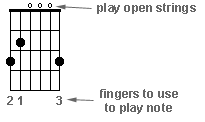
\includegraphics{partone/opengmajor.png}

This diagram illustrates the first chord we are going to play, a G major chord
(often simply called a \term{G chord}). Take your second finger, and put it on the
third fret of the sixth string. Next, take your first finger, and put it on the
second fret of the fifth string. Lastly, put your third finger on the third
fret of the first string. Make sure all of your fingers are curled, and are not
touching any strings they're not supposed to. Now, using your pick, strike all
six strings in one fluid motion. Notes should ring all together, not one at a
time (this could take some practice). Voila! Your first chord.

Now, check to see how you did. While still holding down the chord with your
fretting hand, play each string (starting with the sixth) one at a time,
listening to be sure each note rings out clearly. If not, study your hand to
determine why it doesn't. Are you pressing hard enough? Is one of your other
fingers touching that string, which is preventing it from sounding properly?
These are the most common reasons why a note does not sound. If you're have
trouble, read this feature on getting your chords to ring clearly. 

\subsection{Playing a C major chord}
% image of Cmajor
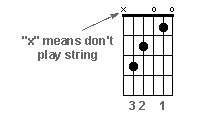
\includegraphics{partone/opencmajor.png}

The second chord we'll learn, the C major chord (often called a \term{C chord}), is
no more difficult than the first G major chord.

Place your third finger on the third fret of the fifth string. Now, put your
second finger on the second fret of the fourth string. Finally, put your first
finger on the first fret of the second string.

Here's where you have to be slightly careful. When playing a C major chord, you
do NOT want to strum the sixth string. Watch your pick to make sure you only
strum the bottom five strings when you are first learning the C major chord.
Test this chord as you did with the G major chord, to make sure all notes are
ringing clearly. 

\subsection{Playing a D major chord}
% image  of Dmajor
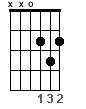
\includegraphics{partone/opendmajor.png}

Some beginners have slightly more difficulty playing a D major chord (often
called a \term{D chord}), since your fingers have to cram into a fairly small area.
Shouldn't be too much of a problem, however, if you can comfortably play the
other two chords.

Place your first finger on the second fret of the third string. Then, put your
third finger on the third fret of the second string. Lastly, place your second
finger on the second fret of the first string. Strum only the bottom 4 strings
when playing a D major chord.

Spend some time familiarizing yourself with these three chords\ldots{} you will use
them for the rest of your guitar-playing career. Make sure you can play each of
the chords without looking at the diagrams. Know what the name of each chord
is, where each finger goes, and which strings you strum or do not strum. 

\section{Learning Songs}
We now know three chords: G major, C major, and D major. Let's see if we can
put them to use in a song. At first, switching chords will take far too long to
be able to play any songs properly. Don't give up, though! With a bit of
practice, you'll be playing away, sounding great (this tutorial on switching
chords quickly might also be of some help). In our next lesson, we'll start
learning about strumming, so you can come back to these songs, and be able to
play them better.

Here are a few of the songs you can play with G major, C major, and D major chords: 

\nameref{sec:song1} --- performed by John Denver

\emph{Notes} when playing the G and C chord, strum them 4 times each, but when
playing the D chord, strum it 8 times

\nameref{sec:song2} --- performed by Kenny Rogers

\emph{Notes} these aren't the exact chords for the song, but they'll do for
now. Try strumming each chord one time, letting them ring.

\nameref{sec:song3} --- performed by Van Morrison

\emph{Notes} There is one chord in this song that we don't know yet, but it's
only used briefly. Skip it for now. Try strumming each chord four times.

\section{Practice Schedule}
Realistically, to start improving on guitar, you're going to need to set aside
a bit of time to practice. Developing a daily routine is a good idea\ldots{}
planning to spend at least 15 minutes daily practicing all you've learned will
really help. At first, your fingers will be sore, but by playing daily, they'll
toughen up, and in a short amount of time, they'll stop hurting. The following
list should give you an idea of how to spend your practice time:
%
\begin{itemize}
\item Get your guitar in tune.
\item Make sure you're sitting, holding the guitar, and using your pick
      properly. You'll have to correct your natural bad habits at first, until it
      becomes second nature.
\item Play the chromatic scale several times. Try playing it backwards.
\item Play each of the three chords you've learned. Check to be sure each note
      is ringing. If not, find out why, and correct the problem.
\item Try moving from one chord to another. Before switching chords, mentally
      picture exactly where each finger is going to move in order to play the next
      chord. Only then should you switch chords. This is the key to switching chords
      quickly. 
\item If you're having trouble getting your chords to ring clearly, read this
      feature on getting your chords to ring clearly.
\item Try playing some, or all of the songs listed above. At first, try only to
      think of the songs as a way in which to practice playing chords.
\item Don't get discouraged. This is hard stuff at first, and you'll probably
      feel like you can't do it. You certainly can. Everyone struggles, so just put
      in your 15 minutes, and then don't worry about it until the next time you play.
      This is supposed to be fun! 
\end{itemize}
%
That's it for now! Once you're comfortable with this lesson, move on to lesson
two, which includes information on the names of the guitar strings, plus more
chords, more songs, and even several basic strumming patterns. Good luck, and
have fun! 

